\documentclass[11pt,a4paper]{article}
\usepackage[utf8]{inputenc}
\usepackage[italian]{babel}
\usepackage{amsmath}
\usepackage{graphicx}
\usepackage{geometry}
\geometry{a4paper, margin=2.5cm}
\usepackage{float}
\usepackage[hypcap=true]{caption}
\usepackage[colorlinks=true, linkcolor=blue, urlcolor=blue]{hyperref}

\title{Relazione Finale - Modellazione e Simulazioni Numeriche \\ \large Progetto sulla Percolazione in 2D e Algoritmo di Hoshen-Kopelman}
\author{Martin Trajkovski}
\date{\today}

\begin{document}

\maketitle

\section{Introduzione e Obiettivi del Progetto}
Questa relazione descrive lo studio condotto sul modello della "Percolazione 2D", analizzato su una griglia quadrata di dimensioni $L \times L$. L'obiettivo principale del lavoro non è stato solo quello di osservare visivamente come si formano i cluster di quadratini "accesi", ma di estrarre dei dati statistici significativi che confermino le leggi fisiche delle transizioni di fase.

In particolare, l'attenzione si è spostata dall'osservazione del singolo reticolo allo studio di grandezze medie calcolate su un gran numero di simulazioni. Per rendere possibile questo studio in tempi ragionevoli, è stato necessario abbandonare l'algoritmo di ricerca classico (\textit{Flood-Fill}), che diventa estremamente lento vicino alla soglia critica, in favore del più efficiente algoritmo di \textit{Hoshen-Kopelman} (HK).

\section{Efficienza Algoritmica: da Flood-Fill a Hoshen-Kopelman}
Il metodo standard per identificare i cluster (implementato in \texttt{CercaCluster.m}) si basa su una ricerca ricorsiva. Questo approccio funziona bene per griglie vuote, ma quando la probabilità di occupazione $p$ si avvicina al valore critico $p_c \approx 0.59$, i cluster diventano molto grandi e ramificati. In queste condizioni, l'algoritmo ricorsivo satura rapidamente la memoria del calcolatore e richiede tempi di calcolo eccessivi.

Per superare questo limite, ho implementato l'algoritmo di \textit{Hoshen-Kopelman}. A differenza del precedente, questo metodo analizza la griglia con un'unica scansione (come se leggesse un libro, riga per riga), assegnando delle etichette temporanee ai quadratini e gestendo i collegamenti tra di essi tramite una struttura dati chiamata \textit{Union-Find}. In questo modo, il tempo richiesto per analizzare la griglia cresce in modo lineare rispetto al numero totale di pixel ($L^2$), rendendo le simulazioni molto veloci.

\begin{figure}[H]
    \centering
    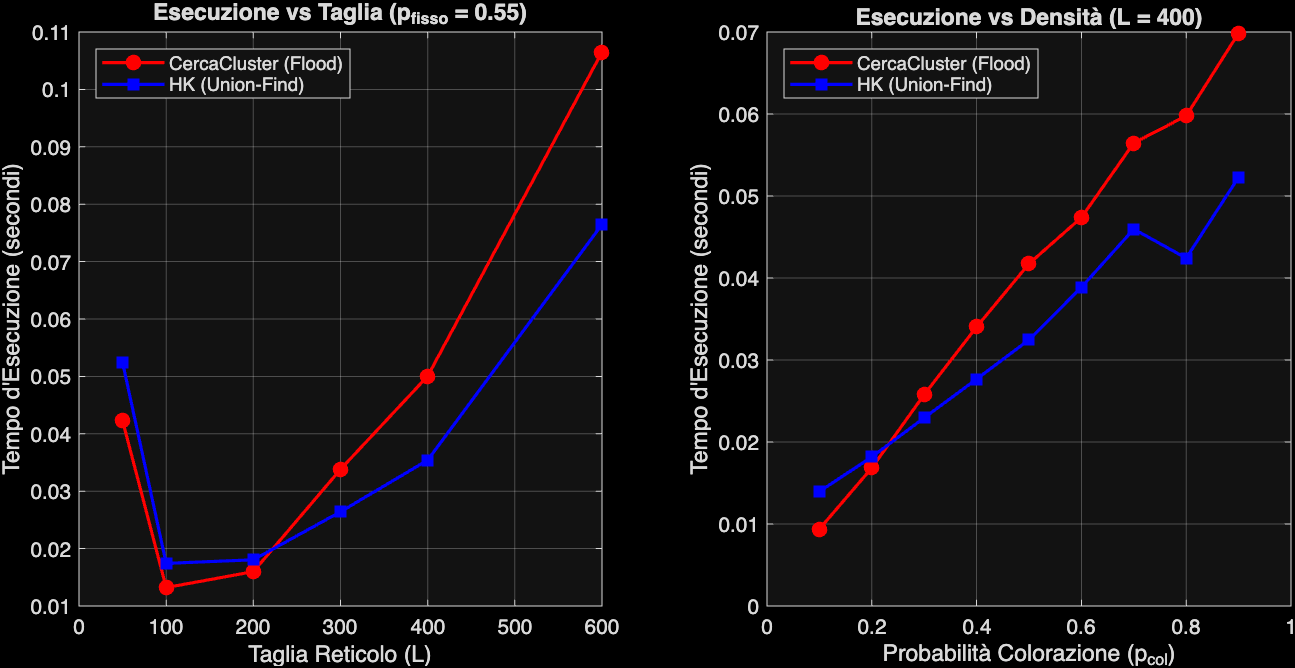
\includegraphics[width=0.9\textwidth]{../Laboratorio_Matlab/Test_efficienza.png}
    \caption{Confronto dei tempi di esecuzione: l'algoritmo Hoshen-Kopelman mantiene prestazioni costanti anche al crescere della complessità del reticolo.}
    \label{fig:efficienza}
\end{figure}

Come si può osservare nella \hyperref[fig:efficienza]{Figura \ref*{fig:efficienza}}, il divario tra i due metodi è netto: mentre il \textit{Flood-Fill} rallenta drasticamente vicino alla soglia di percolazione, l'approccio HK permette di gestire senza problemi griglie di grandi dimensioni.

\section{Analisi dei Risultati: Probabilità, $P_1$ e RACS}
Grazie alla velocità dell'algoritmo HK, ho potuto condurre una campagna di simulazioni molto densa, effettuando $N=1000$ prove per ogni valore di probabilità $p$. Questo ha permesso di ridurre l'errore statistico e di ottenere curve molto pulite.

\begin{figure}[H]
    \centering
    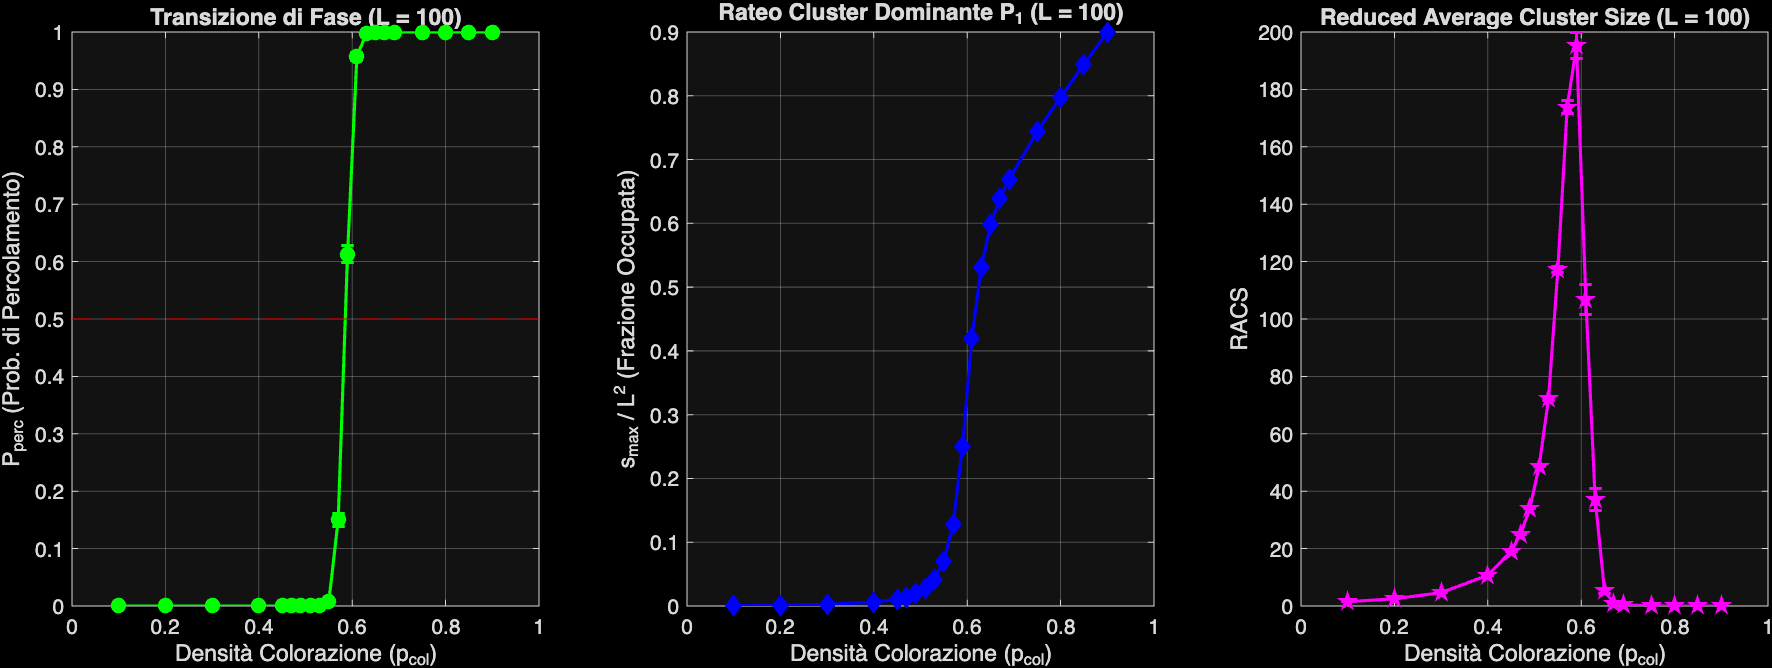
\includegraphics[width=\textwidth]{../Laboratorio_Matlab/analisi_soglia_racs_1000.png}
    \caption{Risultati della simulazione: (1) Probabilità di percolazione, (2) Frazione della massa nel cluster gigante $P_1$, (3) Dimensione media dei cluster ridotta (RACS).}
    \label{fig:termodinamica}
\end{figure}

Dall'analisi dei grafici in \hyperref[fig:termodinamica]{Figura \ref*{fig:termodinamica}} emergono tre punti chiave:
\begin{enumerate}
    \item \textbf{La curva a "S" della percolazione:} La probabilità che esista un cammino che attraversa tutto il sistema non passa da 0 a 1 all'improvviso (come farebbe in un sistema infinito), ma segue una curva più morbida. Il punto di massima pendenza si trova intorno a $p \approx 0.593$, che è in ottimo accordo con i valori teorici della letteratura.
    \item \textbf{Il parametro d'ordine $P_1$:} Questo valore rappresenta la frazione di quadratini che appartengono al cluster più grande. Si nota chiaramente che, superata la soglia critica, questo valore inizia a crescere rapidamente: il "cluster gigante" inizia a fagocitare quasi tutta la massa del sistema.
    \item \textbf{Il picco del RACS (Il "Vulcano"):} Il RACS misura la dimensione media di tutti i cluster esclusione fatta per quello gigante. Rimuovendo il cluster più grande, riusciamo a vedere chiaramente cosa succede agli altri: proprio sulla soglia di percolazione, i cluster diventano molto grandi prima di unirsi tra loro, creando un picco caratteristico nel grafico.
\end{enumerate}

\section{Conclusioni e Osservazioni di Studio}
\subsection*{4.1 Effetti di taglia finita (Finite-Size Scaling)}
Sebbene la teoria preveda un salto netto (funzione di Heaviside) per la percolazione, nelle mie simulazioni ho usato una griglia di lato $L=100$. Questa dimensione "finita" è responsabile dell'arrotondamento della curva a S. In una griglia reale di un computer, i bordi influenzano il risultato: un sistema infinito non ha bordi, mentre qui i cluster che toccano i lati del riquadro vengono considerati "percolanti" un po' prima del previsto.

\subsection*{4.2 Affidabilità dei dati}
L'utilizzo del metodo Monte Carlo indipendente (rigenerando la griglia da zero per ogni prova) garantisce che non vi sia alcuna correlazione tra un esperimento e l'altro. Avendo utilizzato $1000$ medie per punto, i risultati ottenuti sono statisticamente solidi e l'errore calcolato (tramite la deviazione standard della media) è estremamente contenuto, confermando la bontà del modello implementato in \texttt{Matlab}.

\end{document}
